\documentclass[14pt]{extbook}
\usepackage{multicol, enumerate, enumitem, hyperref, color, soul, setspace, parskip, fancyhdr} %General Packages
\usepackage{amssymb, amsthm, amsmath, latexsym, units, mathtools} %Math Packages
\everymath{\displaystyle} %All math in Display Style
% Packages with additional options
\usepackage[headsep=0.5cm,headheight=12pt, left=1 in,right= 1 in,top= 1 in,bottom= 1 in]{geometry}
\usepackage[usenames,dvipsnames]{xcolor}
\usepackage{dashrule}  % Package to use the command below to create lines between items
\newcommand{\litem}[1]{\item#1\hspace*{-1cm}\rule{\textwidth}{0.4pt}}
\pagestyle{fancy}
\lhead{Progress Quiz 10}
\chead{}
\rhead{Version A}
\lfoot{5170-5105}
\cfoot{}
\rfoot{Summer C 2021}
\begin{document}

\begin{enumerate}
\litem{
Solve the linear equation below. Then, choose the interval that contains the solution.\[ \frac{7x -8}{4} - \frac{9x + 5}{8} = \frac{5x -7}{7} \]\begin{enumerate}[label=\Alph*.]
\item \( x \in [-68.2, -66.2] \)
\item \( x \in [-2.23, 2.77] \)
\item \( x \in [-22.2, -15.2] \)
\item \( x \in [-5.2, -2.2] \)
\item \( \text{There are no real solutions.} \)

\end{enumerate} }
\litem{
Write the equation of the line in the graph below in Standard Form $Ax+By=C$. Then, choose the intervals that contain $A, B, \text{ and } C$.
\begin{center}
    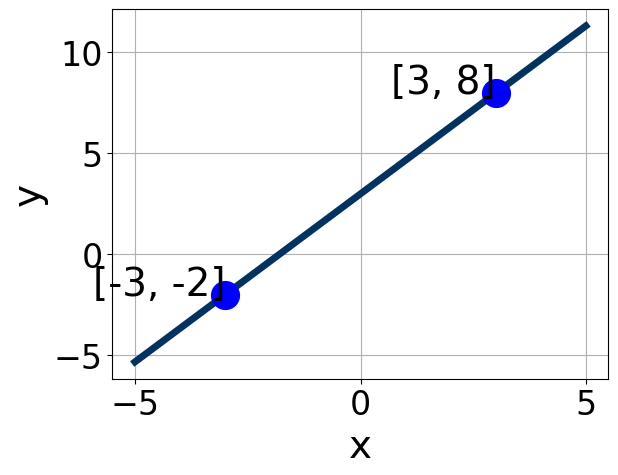
\includegraphics[width=0.5\textwidth]{../Figures/linearGraphToStandardCopyA.png}
\end{center}
\begin{enumerate}[label=\Alph*.]
\item \( A \in [5, 8], \hspace{3mm} B \in [1.24, 3.48], \text{ and } \hspace{3mm} C \in [7.4, 9.5] \)
\item \( A \in [-2.67, 3.33], \hspace{3mm} B \in [-2.13, -0.61], \text{ and } \hspace{3mm} C \in [-4.5, -2.9] \)
\item \( A \in [5, 8], \hspace{3mm} B \in [-3.76, -1.94], \text{ and } \hspace{3mm} C \in [-9.2, -7.4] \)
\item \( A \in [-2.67, 3.33], \hspace{3mm} B \in [0.53, 1.28], \text{ and } \hspace{3mm} C \in [1.3, 3.4] \)
\item \( A \in [-7, -4], \hspace{3mm} B \in [1.24, 3.48], \text{ and } \hspace{3mm} C \in [7.4, 9.5] \)

\end{enumerate} }
\litem{
Find the equation of the line described below. Write the linear equation in the form $ y=mx+b $ and choose the intervals that contain $m$ and $b$.\[ \text{Parallel to } 9 x - 5 y = 11 \text{ and passing through the point } (-8, 8). \]\begin{enumerate}[label=\Alph*.]
\item \( m \in [0.9, 2.6] \hspace*{3mm} b \in [15, 18] \)
\item \( m \in [0.9, 2.6] \hspace*{3mm} b \in [-22.4, -20.4] \)
\item \( m \in [-2.8, -1.2] \hspace*{3mm} b \in [-9.4, -1.4] \)
\item \( m \in [-0.1, 1.2] \hspace*{3mm} b \in [21.4, 24.4] \)
\item \( m \in [0.9, 2.6] \hspace*{3mm} b \in [21.4, 24.4] \)

\end{enumerate} }
\litem{
Solve the equation below. Then, choose the interval that contains the solution.\[ -7(-19x -4) = -10(-2x -15) \]\begin{enumerate}[label=\Alph*.]
\item \( x \in [1.14, 1.63] \)
\item \( x \in [0.78, 1.1] \)
\item \( x \in [-1.34, -0.95] \)
\item \( x \in [-1.7, -1.34] \)
\item \( \text{There are no real solutions.} \)

\end{enumerate} }
\litem{
Find the equation of the line described below. Write the linear equation in the form $ y=mx+b $ and choose the intervals that contain $m$ and $b$.\[ \text{Parallel to } 5 x + 3 y = 4 \text{ and passing through the point } (-10, 7). \]\begin{enumerate}[label=\Alph*.]
\item \( m \in [-2.68, -1.16] \hspace*{3mm} b \in [-12.67, -1.67] \)
\item \( m \in [-2.68, -1.16] \hspace*{3mm} b \in [7.67, 12.67] \)
\item \( m \in [-0.34, 2.7] \hspace*{3mm} b \in [22.67, 24.67] \)
\item \( m \in [-2.68, -1.16] \hspace*{3mm} b \in [17, 21] \)
\item \( m \in [-1.51, -0.19] \hspace*{3mm} b \in [-12.67, -1.67] \)

\end{enumerate} }
\litem{
Solve the linear equation below. Then, choose the interval that contains the solution.\[ \frac{-3x + 9}{5} - \frac{-5x + 5}{2} = \frac{6x + 7}{4} \]\begin{enumerate}[label=\Alph*.]
\item \( x \in [-6.38, -3.38] \)
\item \( x \in [7.5, 10.5] \)
\item \( x \in [-2.61, 0.39] \)
\item \( x \in [3.13, 7.13] \)
\item \( \text{There are no real solutions.} \)

\end{enumerate} }
\litem{
First, find the equation of the line containing the two points below. Then, write the equation in the form $ y=mx+b $ and choose the intervals that contain $m$ and $b$.\[ (-6, -3) \text{ and } (10, -8) \]\begin{enumerate}[label=\Alph*.]
\item \( m \in [-0.81, -0.1] \hspace*{3mm} b \in [2.1, 3.4] \)
\item \( m \in [-0.81, -0.1] \hspace*{3mm} b \in [4.4, 7] \)
\item \( m \in [-0.81, -0.1] \hspace*{3mm} b \in [-19.2, -17] \)
\item \( m \in [-0.81, -0.1] \hspace*{3mm} b \in [-6.2, -4.4] \)
\item \( m \in [-0.2, 0.42] \hspace*{3mm} b \in [-11.9, -11.1] \)

\end{enumerate} }
\litem{
Write the equation of the line in the graph below in Standard Form $Ax+By=C$. Then, choose the intervals that contain $A, B, \text{ and } C$.
\begin{center}
    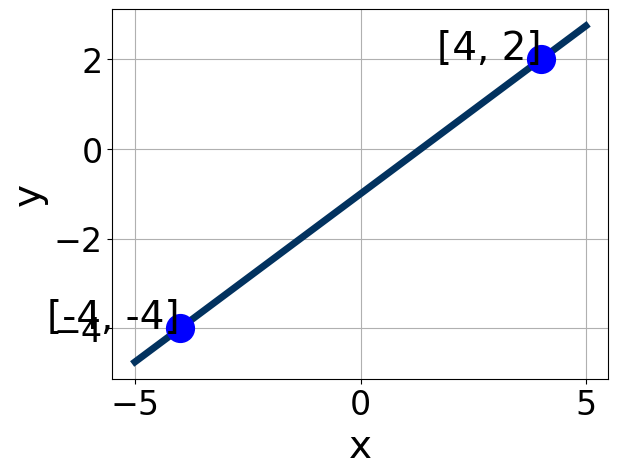
\includegraphics[width=0.5\textwidth]{../Figures/linearGraphToStandardA.png}
\end{center}
\begin{enumerate}[label=\Alph*.]
\item \( A \in [-1.7, 2.6], \hspace{3mm} B \in [0.2, 2.1], \text{ and } \hspace{3mm} C \in [-1.5, -0.4] \)
\item \( A \in [-3.8, -1.5], \hspace{3mm} B \in [2.6, 4.3], \text{ and } \hspace{3mm} C \in [-5.2, -3.5] \)
\item \( A \in [-1.7, 2.6], \hspace{3mm} B \in [-3.2, -0.2], \text{ and } \hspace{3mm} C \in [-0.4, 2.3] \)
\item \( A \in [1.8, 3.1], \hspace{3mm} B \in [-5.6, -1.8], \text{ and } \hspace{3mm} C \in [2.8, 4.9] \)
\item \( A \in [1.8, 3.1], \hspace{3mm} B \in [2.6, 4.3], \text{ and } \hspace{3mm} C \in [-5.2, -3.5] \)

\end{enumerate} }
\litem{
First, find the equation of the line containing the two points below. Then, write the equation in the form $ y=mx+b $ and choose the intervals that contain $m$ and $b$.\[ (5, 7) \text{ and } (2, 6) \]\begin{enumerate}[label=\Alph*.]
\item \( m \in [-0.2, 1.5] \hspace*{3mm} b \in [-0.43, 3.03] \)
\item \( m \in [-0.2, 1.5] \hspace*{3mm} b \in [3.69, 4.44] \)
\item \( m \in [-0.2, 1.5] \hspace*{3mm} b \in [4.59, 5.78] \)
\item \( m \in [-0.2, 1.5] \hspace*{3mm} b \in [-6.33, -5.05] \)
\item \( m \in [-2.3, -0.1] \hspace*{3mm} b \in [6.03, 7.9] \)

\end{enumerate} }
\litem{
Solve the equation below. Then, choose the interval that contains the solution.\[ -6(-4x + 9) = -3(-8x -17) \]\begin{enumerate}[label=\Alph*.]
\item \( x \in [-0.04, 0.05] \)
\item \( x \in [0.05, 0.1] \)
\item \( x \in [-0.04, 0.05] \)
\item \( x \in [-0.04, 0.05] \)
\item \( \text{There are no real solutions.} \)

\end{enumerate} }
\end{enumerate}

\end{document}